\documentclass[../main.tex]{subfiles}
\begin{document}\label{appendixC}

Chương \ref{chap4} đã phát biểu các công thức cho xác suất truyền tin tại PU và SU trong trường hợp hợp tác, cụ thể:
\begin{subequations}\label{proofC:ptx}
\begin{align}
p_{tx}^{(P)} 
    &= \frac{p_P\Omega_{pp}}{p_S\Omega_{sp}\gamma_b^{(P)} + p_P\Omega_{pp}}\exp\left(-\frac{\gamma_b^{(P)}N_P}{p_P\Omega_{pp}}\right), \label{proofC:ptxp} \\
p_{tx}^{(S)} 
    &= \frac{p_S\Omega_{ss}}{p_P\Omega_{ps}\gamma_b^{(S)} + p_S\Omega_{ss}}\exp\left(-\frac{\gamma_b^{(S)}N_S}{p_S\Omega_{ss}}\right).\label{proofC:ptxs}
\end{align}
\end{subequations}
Phần này thực hiện khảo sát các công thức trên, từ đó xác định dải giá trị cho các tham số tùy chỉnh $\sigma^{(P)}$ và $\sigma^{(S)}$ trong bài toán tối ưu đề xuất trong Chương \ref{chap3}.

\section{Giá trị lớn nhất của xác suất truyền tin}

Trong các công thức xác suất truyền tin của PU và SU, các công suất phát $p_P$ và $p_S$ là các biến có thể thay đổi và các tham số còn lại là xác định trước đối với một điều kiện truyền tin cụ thể. Do đó, ta đi khảo sát hàm hai biến sau:
\begin{equation}\label{fptx}
    p\left(x, y; a, b\right) = \frac{x}{ay+x}\exp\left(-\frac{b}{x}\right),
\end{equation}
với $a, b$ là các hằng số dương, $x, y$ là các biến thực, $x > 0, y \geq 0$. Khi đó, các đạo hàm riêng của $p$ có công thức như sau:
\begin{subequations}
\begin{align}
\frac{\partial{p}}{\partial{x}} &= \frac{\exp\left(-\frac{b}{x}\right)}{\left(ay+x\right)^2}\left(ay + b + ab\frac{y}{x}\right),  \\
\frac{\partial{p}}{\partial{y}} &= \frac{\exp\left(-\frac{b}{x}\right)}{\left(ay+x\right)^2}\left(-a\right).
\end{align}
\end{subequations}
Do $a, b, x$ đều dương và $y \geq 0$ nên ${\partial{p}}/{\partial{x}} > 0$ và ${\partial{p}}/{\partial{y}} < 0$. Điều đó cho thấy $p$ là hàm đồng biến theo $x$ và nghịch biến theo $y$. Như vậy, giá trị lớn nhất của $p$ đạt được khi $y = 0$ và $x$ nhận giá trị lớn nhất, $x = x_{max}$, giá trị của $p$ khi đó là:
\begin{equation*}
    \max_{x,y}\left\{p\right\} = \exp\left(-\frac{b}{x_{max}}\right).
\end{equation*}
Khi $x$ không bị chặn trên, dễ thấy, $\max_{x,y}\left\{p\right\} = 1$.

Các công thức xác suất truyền tin \eqref{proofC:ptxp} và \eqref{proofC:ptxs} có thể được viết lại theo hàm $p$ định nghĩa trong \eqref{proofC:ptx} thành:
\begin{subequations}\label{proofC:ptxrw}
\begin{align}
p_{tx}^{(P)} &= p\left(p_P, p_S; \frac{\gamma_b^{(P)}\Omega_{sp}}{\Omega_{pp}}, \frac{\gamma_b^{(P)}N_P}{\Omega_{pp}}\right), \label{proofC:ptxprw} \\
p_{tx}^{(S)} &= p\left(p_S, p_P; \frac{\gamma_b^{(S)}\Omega_{ps}}{\Omega_{ss}}, \frac{\gamma_b^{(S)}N_S}{\Omega_{ss}}\right). \label{proofC:ptxsrw}
\end{align}
\end{subequations}
Như vậy, xác suất truyền tin cực đại tại các bên tương ứng là:
\begin{subequations}\label{proofC:ptxmax}
\begin{align}
\max_{p_P, p_S}\left\{p_{tx}^{(P)}\right\} &= \exp\left(-\frac{\gamma_b^{(P)}N_P}{p_P^{max}\Omega_{pp}}\right), \\
\max_{p_P, p_S}\left\{p_{tx}^{(S)}\right\} &= \exp\left(-\frac{\gamma_b^{(S)}N_S}{p_S^{max}\Omega_{ss}}\right).
\end{align}
\end{subequations}

Ngoài ra, từ kết quả khảo sát hàm $p$, ta thấy $p_{tx}^{(P)}$ tỷ lệ thuận với $p_P$ và tỷ lệ nghịch với $p_S$, ngược lại $p_{tx}^{(S)}$ tỷ lệ thuận với $p_S$ và tỷ lệ nghịch với $p_P$. Tức là nếu thay đổi $p_P$ và $p_S$ để tăng giá trị $p_{tx}^{(P)}$ thì giá trị $p_{tx}^{(S)}$ sẽ giảm, cả hai bên không thể cùng đạt được xác suất truyền tin quá cao.

\section{Điều kiện để các bên đạt được xác suất truyền tin mong muốn}

Bài toán thiết kế \eqref{moop}, mặc dù do SU giải quyết, nhưng PU lại có quyền ưu tiên hơn trong việc xác định các tham số của mình, đó là $R_b^{(P)}$, $R_s^{(P)}$, $p_P^{max}$ và đặc biệt là $\sigma^{(P)}$. Nếu đề xuất của SU không đảm bảo các yêu cầu đó thì SU không thể được chọn cùng truyền với PU. Do đó, trong bài toán thiết kế của mình, SU không thể tùy ý lựa chọn các tham số. Khi PU xác định trước yêu cầu về xác suất truyền tin tối thiểu $\sigma^{(P)}$, nếu muốn hợp tác cùng truyền với PU, SU chỉ có thể lựa chọn một giá trị $\sigma^{(S)}$ đảm bảo cho tập $G$ khác rỗng, với $G$ được định nghĩa bởi:
\begin{equation}\label{proofC:set}
    G = \left\{\left(p_P, p_S\right)\Bigl|p_{tx}^{(P)} \geq \sigma^{(P)}, p_{tx}^{(S)} \geq \sigma^{(S)}, 0 < p_P \leq p_P^{max}, 0 < p_S \leq p_S^{max} \right\}.
\end{equation}
Tập $G$ đại diện cho các lựa chọn công suất phát của PU và SU đảm bảo cả hai bên cùng đạt được xác suất truyền tin tối thiểu mong muốn, tương ứng là $\sigma^{(P)}$ và $\sigma^{(S)}$. Dễ thấy, tập $G$ cũng chính là tập các giá trị hợp lệ của các biến quyết định trong bài toán tối ưu \eqref{moop}. Tập $G$ rỗng đồng nghĩa SU không thể đề xuất bất kỳ chiến lược xác định công suất phát nào tới PU, và hai bên không thể hợp tác. Khi giá trị $p_{tx}^{(S)}$ càng tăng thì $p_{tx}^{(P)}$ càng giảm, từ đó điều kiện $p_{tx}^{(P)} \geq \sigma^{(P)}$ càng khó đạt được. Như vậy, khi SU càng yêu cầu cao về xác suất truyền tin tối thiểu thì lực lượng tập $G$ càng giảm. Do đó, phần này thực hiện tìm giá trị lớn nhất của $\sigma^{(S)}$ đảm bảo tập $G$ khác rỗng, khi $\sigma^{(P)}$ cố định.

Trước hết, từ \eqref{proofC:ptx}, các điều kiện $p_{tx}^{(P)} \geq \sigma^{(P)}$ và $p_{tx}^{(S)} \geq \sigma^{(S)}$ biểu diễn lại theo $p_P$ và $p_S$ như sau:
\begin{subequations}\label{proofC:gp}
\begin{align}
p_S \leq \frac{p_P\Omega_{pp}}{\Omega_{sp}\gamma_b^{(P)}}
\left(\frac{1}{\sigma^{(P)}}\exp\left(-\frac{\gamma_b^{(P)}N_P}{p_P\Omega_{pp}}\right) - 1\right), \\
p_P \leq \frac{p_S\Omega_{ss}}{\Omega_{ps}\gamma_b^{(S)}}
\left(\frac{1}{\sigma^{(S)}}\exp\left(-\frac{\gamma_b^{(S)}N_S}{p_S\Omega_{ss}}\right) - 1\right).
\end{align}
\end{subequations}

Từ đó, ta khảo sát hàm $\phi\left(x;a,b,c\right)$ phụ thuộc vào biến $x$ dương và các hằng số thực dương $a,b,c$ và $b \geq 1$ được định nghĩa như sau:
\begin{equation}\label{proofC:g}
    \phi\left(x;a,b,c\right) = ax\left(b\exp\left(-\frac{c}{x}\right)-1\right).
\end{equation}
Đạo hàm bậc một và bậc hai của $\phi$ theo biến $x$ có công thức như sau:
\begin{subequations}\label{proofC:dg}
\begin{align}
\phi'\left(x\right) &= ab\exp\left(-\frac{c}{x}\right)\left(1+\frac{c}{x}\right)-a, \\
\phi''\left(x\right) &= ab\exp\left(-\frac{c}{x}\right)\frac{c^2}{x^3}. 
\end{align}
\end{subequations}
Do $a,b,c$ dương nên $\phi''\left(x\right) > 0, \forall x > 0$. Ngoài ra, từ công thức định nghĩa, ta thấy phương trình $\phi\left(x;a,b,c\right) = 0$ có nghiệm dương duy nhất $x^* = c/\ln{b}$ và $\phi(x) < 0, \forall x<x^*$. Đồng thời, do $\phi''(x) > 0, \forall x > 0$ nên ta có $\phi'(x) \geq \phi'(x^*) > 0, \forall x \geq x^*$. Điều đó cho thấy, $\phi$ là hàm đồng biến trên khoảng $\left[x^*, \infty\right)$, nên ta có $\phi(x) \geq \phi(x^*) = 0, \forall x \geq x^*$.  Tóm lại, $\phi(x)$ có ba tính chất quan trọng sau đây: (i) có nghiệm dương duy nhất $x^*$, (ii) đồng biến trên khoảng  $\left[x^*,\infty\right)$ và (iii) $\phi(x) \geq 0$ khi và chỉ khi $x \geq x^*$.

Dựa trên hàm $\phi$ trong \eqref{proofC:g}, các công thức \eqref{proofC:gp} trở thành:
\begin{subequations}\label{proofC:gprw}
\begin{align}
p_S \leq \phi\left(p_P; \frac{\Omega_{pp}}{\Omega_{sp}\gamma_b^{(P)}}, \frac{1}{\sigma^{(P)}}, \frac{\gamma_b^{(P)}N_P}{\Omega_{pp}}\right) =  \phi_p\left(p_P\right), \\
p_P \leq \phi\left(p_S; \frac{\Omega_{ss}}{\Omega_{ps}\gamma_b^{(S)}}, \frac{1}{\sigma^{(S)}}, \frac{\gamma_b^{(S)}N_S}{\Omega_{ss}}\right) = \phi_s\left(p_S\right).
\end{align}
\end{subequations}
Từ đó, ta có thể biểu diễn tập $G$ trên hệ trục tọa độ như Hình~\ref{fig:Constraints}. Dễ thấy rằng, tập $G$ khác rỗng khi và chỉ khi hai đường cong $p_S = \phi_p\left(p_P\right)$ và $p_P = \phi_s\left(p_S\right)$ cắt nhau tại một điểm $S$ nằm trong hình chữ nhật $OABC$ với tọa độ 4 đỉnh lần lượt là $\left(0, 0\right)$, $\left(0, p_S^{max}\right)$, $\left(p_P^{max}, p_S^{max}\right)$ và $\left(p_P^{max}, 0\right)$. 

\begin{figure}
\centering
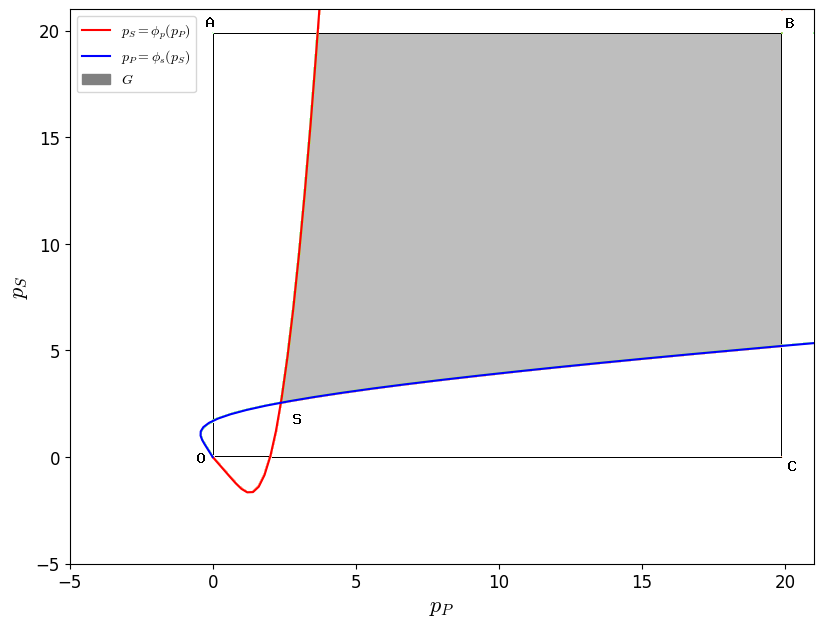
\includegraphics[width=0.8\linewidth]{constraints.png}
\caption{Tập $G$ (phần bôi đậm) biểu diễn theo $p_P$ và $p_S$ với $p_P^{max}=20$, $p_S^{max}=20$}
\label{fig:Constraints}
\end{figure}

Gọi tọa độ của điểm $S$ là $\left(p_P^*, p_S^*\right)$, tức là ta có $p_S^* = \phi_p\left(p_P^*\right)$ và $p_P^* = \phi_s\left(p_S^*\right)$. Do $p_P^* > 0$ nên $\phi_s\left(p_S^*\right) > 0$, theo tính chất của hàm $\phi$, điều kiện này chỉ xảy ra khi $p_S^* > p_S^z$ với $p_S^z$ là nghiệm của $\phi_s(x) = 0$. Tương tự, ta có $p_P^* > p_P^z$, với $p_P^z$ là nghiệm của $\phi_p(x) = 0$. Đây là các giới hạn dưới cho $p_P^*$ và $p_S^*$. Đồng thời, ta có $p_P^*$ là nghiệm của phương trình $\Phi_p\left(x\right) = 0$ với:
\begin{equation}\label{proofC:Phip}
\Phi_p\left(x\right) = \phi_s\left(\phi_p\left(x\right)\right) - x,
\end{equation}
và $p_S^*$ là nghiệm của phương trình $\Phi_s\left(x\right) = 0$ với:
\begin{equation}\label{proofC:Phis}
\Phi_s\left(x\right) = \phi_p\left(\phi_s\left(x\right)\right) - x.
\end{equation}
Tiếp theo, ta đi khảo sát hàm $\Phi_p$ và $\Phi_s$ trên các khoảng $\left(p_P^z, p_P^{max}\right]$ và $\left(p_S^z, p_S^{max}\right]$ tương ứng.

Không mất tổng quát, ta đi khảo sát hàm $\Phi \equiv \Phi_p$ trên miền $\left(x_p, \infty\right)$, với $x_p$ là nghiệm dương của phương trình $\phi_p(x)=0$. Đạo hàm cấp một và cấp hai của $\Phi$ có công thức sau:
\begin{subequations}\label{proofC:dPhi}
\begin{align}
\Phi'(x) &= \phi_p'(x).\phi_s'(\phi_p(x)) - 1,  \\
\Phi''(x) &= \phi_p''(x).\phi_s'(\phi_p(x)) 
+ \phi_p'(x)^2.\phi_s''(\phi_p(x)). \label{proofC:ddPhi}
\end{align}
\end{subequations}
Gọi $x_0$ là nghiệm của phương trình $\phi_p(x) = x_s$ trên khoảng $\left(x_{p}, \infty\right)$, với $x_s$ là nghiệm dương duy nhất của phương trình $\phi_s(x)=0$. Dễ thấy, $x_0$ luôn tồn tại vì $\phi_p(x)$ nhận giá trị trên khoảng $\left(0, \infty\right)$ khi $x$ biến thiên trên $\left(x_{p}, \infty\right)$. Khi đó, ta có $\phi_s(\phi_p(x_0)) = \phi_s(x_p) = 0$. Từ đó, theo tính chất của hàm $\phi$, ta dễ dàng chứng minh ba mệnh đề sau:
\begin{subequations}
\begin{align}
\phi_s(\phi_p(x)) \geq \phi_s(\phi_p(x_0)) = 0, \forall x \geq x_0, \\
\phi_s'(\phi_p(x)) \geq 0, \forall x \geq x_0, \label{proofC:x0pos} \\
\phi_s(\phi_p(x)) < \phi_s(\phi_p(x_0)) = 0, \forall \ x_{p} < x < x_0. \label{proofC:x0neg}
\end{align}
\end{subequations}
Theo \eqref{proofC:x0neg}, khi $x_{p} < x < x_0$, thì $\Phi(x) < 0$, phương trình $\Phi(x) = 0$ không thể có nghiệm trên khoảng $\left(x_{p}, x_0\right)$. Khi $x \geq x_0$, theo \eqref{proofC:x0pos} và \eqref{proofC:ddPhi}, ta có $\Phi''(x) > 0$. Như vậy, $\Phi$ là hàm lồi trên khoảng $\left[x_0, \infty\right)$. Mà $\Phi(x_0)=-x_0 < 0$, từ đó dễ dàng chứng minh bằng phương pháp phản chứng: (i) phương trình $\Phi(x) = 0$ có nghiệm trên khoảng $\left(x_0, x_1\right]$, $x_1 > x_0$ khi và chỉ khi $\Phi(x_1) \geq 0$ và (ii) nghiệm trên miền xác định của phương trình $\Phi(x) = 0$ là duy nhất (nếu có).

Từ kết quả khảo sát hàm $\Phi$, phương trình $\Phi_p(x)=0$ có nghiệm $p_P^*$ trên khoảng $\left(p_P^z, p_P^{max}\right]$ khi và chỉ khi $\phi_s(\phi_p(p_P^{max})) \geq p_P^{max}$. Tương tự, phương trình $\Phi_s(x)=0$ có nghiệm $p_S^*$ trên khoảng $\left(p_S^z, p_S^{max}\right]$ khi và chỉ khi $\phi_p(\phi_s(p_S^{max})) \geq p_S^{max}$. Đồng thời, các nghiệm này đều là duy nhất (nếu có). Như vậy, $G$ khác rỗng khi và chỉ khi $\phi_s(\phi_p(p_P^{max})) \geq p_P^{max}$ và $\phi_p(\phi_s(p_S^{max})) \geq p_S^{max}$. Bài toán ban đầu được giải quyết.

\end{document}